\section{Opgaver}

\begin{opgave}{Stjernernes spektre}{1}
  Figur \ref{fig:stellar_abs} viser forskellige spektraltyper og visse
  absorptionslinjer angivet.
\begin{figure}[h]
	\centering
	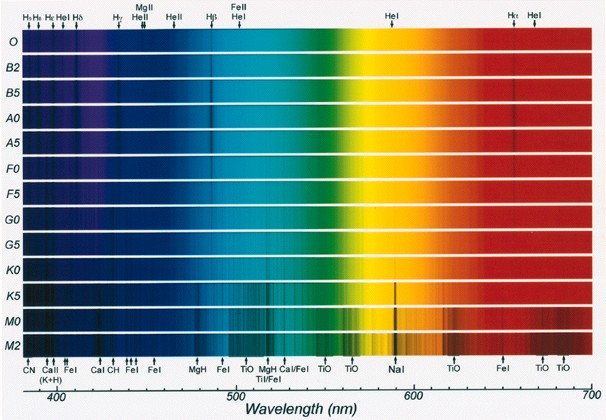
\includegraphics[width=\textwidth]{astro/fig/stellar_abs.jpg}
	\caption{Absorption for spektraltyper.}
	\label{fig:stellar_abs}
\end{figure}
\opg Solen har spektralklasse G2V, men i dette tilfælde kan vi godt
tilnærme den til en G0-type. Hvad er nogle eksempler på grundstoffer,
som kan ses i dens atmosfære?  \opg Stjerner af typerne M0 og M2 har
f.eks. molekylerne MgH og TiO i deres atmosfærer. Ud fra din viden om
spektraltyper hvad vil du så sige var den primære årsag til at
molekylerne kan eksistere i deres atmosfærer?
\end{opgave}

\begin{opgave}{Blinke, blinke stjerne der}{1}
  Stjernen Dschubba i stjernebilledet Skorpionen (som ser virkelig
  nice ud på en mørk nattehimmel men som man skal til Sydeuropa eller
  længere ned for at kunne se) har en overfladetemperatur på 28 000 K,
  en anslået radius på $5,6 \cdot 10^9$ m og ligger i en afstand på
  123 pc. Stjernen har en tilsyneladende magnitude på $m=2,3$ \opg
  Hvad er stjernens luminositet?  \opg Hvad er stjernens flux ved dens
  overflade?  \opg Hvad er stjernens flux ved Jordens overflade?  \opg
  Solen har en tilsyneladende magnitude på $m_\odot=-27$. Hvad er
  stjernens flux i enheder af Solens flux?
\end{opgave}

\begin{opgave}{Afstandsbedømmelse i nabolaget}{2}
	En stjerne har en tilsyneladende magnitude på 17,5 og en absolut magnitude på -1,27.
	\opg Hvad er afstanden til stjernen? 
	\opg Satellitten GAIA som blev opsendt i 2012 kan måle parallakser ned til ca. 20 mikro-buesekunder ($10^{-6}$). Vil GAIA kunne måle stjernens parallakse?
	\opg Det oplyses nu, at lyset på sin vej fra stjernen til os er blevet reduceret med 60pct. pga. udslukning fra interstellart støv. Hvad er den faktiske afstand til stjernen? Kan GAIA måle stjernens parallakse? 
\end{opgave}

\begin{opgave}{Sortlegemestråling}{1}
  Planeter, almindelige stjerner og kompakte objekter er ekspempler på
  objekter, som til en god tilnærmelse kan beskrives som sorte
  legemer. Det betyder, at spektrene for den stråling, de udsender, er
  næsten perfekte Planck-spektre givet ved Plancks strålingslov, og at
  de udstråler med maksimal intensitet ved bølgelængden:

\begin{equation}
\lambda_\text{max} = \frac{2.898 \cdot 10^{6} \SI{}{nm}~\SI{}{K}}{T}
\label{eq:wien}
\end{equation}

%Vi ser på fire objekter:
%\begin{itemize}
%\item En planet med overfladetemperatur $T_\text{p} = 290 \SI{}{K}$
%\item En stjerne med overfladetemperatur $T_\text{s} = 5,0\cdot 10^3 \SI{}{K}$
%\item En hvid dværg med overfladetemperatur $T_\text{hd} = 2,5\cdot 10^4 \SI{}{K}$
%\item En neutronstjerne med overfladetemperatur $T_\text{ns} = 1,0\cdot 10^6 \SI{}{K}$
%\end{itemize}
%%%%% opgave-environment kan ikke finde ud af itemize,når der ikke er tekst inden \opg, derfor mærkeligt pseudo-lister:
Vi ser på fire objekter:\\
 -- En planet med overfladetemperatur $T_\text{p} = 290\, \SI{}{K}$\\
 -- En stjerne med overfladetemperatur $T_\text{s} = 5,0\cdot 10^3\, \SI{}{K}$\\
 -- En hvid dværg med overfladetemperatur $T_\text{hd} = 2,5\cdot 10^4\, \SI{}{K}$\\
 -- En neutronstjerne med overfladetemperatur $T_\text{ns} = 1,0\cdot 10^6\, \SI{}{K}$
\opg Hvilket af de fire objekter udsender sortlegemestråling med den korteste bølgelængde ved maksimal intensitet?
\opg Det oplyses nu at radiierne for de fire objekter er: \\
 -- Planet $R_p = 6000$ km\\
 -- Stjerne $R_s = 6,0\cdot 10^5$ km\\
 -- Hvid dværg $R_{hd} = 6000$ km\\
 -- Neutronstjerne $R_{ns} = 10$ km\\

Hvilket af de fire objekter udsender sortlegemestråling med den største luminositet? 
\end{opgave}

\begin{opgave}{Det super-massive sorte hul i Mælkevejens centrum}{2}
  Stjernen S0-16 er en B-stjerne med en masse omkring 10$M_{\odot}$,
  som bevæger sig i en elliptisk bane omkring et objekt i Mælkevejens
  centrum med den halve storakse $a = 1800$ AU, eccentricitet $e =
  0,9389$ og omløbsperiode $P = 38$ år.  \opg Bestem massen af det
  centrale objekt, som S0-16 er i bane om.  \opg Hvad er den korteste
  afstand i banen mellem S0-16 og det centrale objekt? \emph{Hint: Se
    på figur \ref{fig:ellipsemat}.}  \opg S0-16 er udsat for voldsomme
  tidevandskræfter, når den bevæger sig ind omkring det centrale
  objekt. Vurder hvor meget større tidevandspåvirkningen på S0-16 er i
  periastron i forhold til i det punkt i banen, hvor S0-16 er længst
  fra det centrale objekt. \emph{Hint: Den største afstand i banen er
    det, vi definerer som apoapsis.}  \opg Brug resultaterne til at
  argumentere for, at objektet i centrum af Mælkevejen formentlig er
  et gigantisk sort hul.
\end{opgave}

%\begin{opgave}{M87}{1}
%	\emph{Galaksen M87 ligger i centrum af den nærmeste store galaksehob Virgohoben. Rødforskydningen af lys fra M87 og dermed fra centrum af Virgohoben er målt til $z = 0.00436$. Vi antager en Hubblekonstant på $H_0 = 70$ km/s/Mpc.}
%	\opg 
%	Beregn afstanden til M87. Gør rede for dine antagelser. 
%\end{opgave}

\begin{opgave}{That's no moon...}{3}
  Saturns måne Mimas er placeret i en elliptisk bane omkring Saturn
  med halve storakse $a_\text{Mimas}=185,5\cdot 10^3$ km. Desuden
  oplyses det, at massen af Saturn er $M_s = 5,685\cdot 10^{26}$ kg og
  at massen af Mimas er $M_\text{Mimas} = 3,751\cdot 10^{19}$ kg.  \opg
  Bestem baneperioden for Mimas. \\
  Vi vil nu i de følgende opgaver prøve at udregne temperaturen på
  overfladen af Mimas.  \opg Vis først, at en planet eller måne med
  radius $R_m$ i en afstand $d$ fra Solen og med en albedo-værdi på
  $A$ vil absorbere energien
 \begin{equation}
 L_\text{abs} = \frac{R_\odot^2\sigma T_\odot^4 \pi R_m^2}{d^2} \left( 1 - A \right),
 \end{equation}
 
 hvor $R_\odot$ og $T_\odot$ er hhv. radius og temperatur af Solen. \emph{Hint: man kan sige, at den del af planeten eller månen der er vendt mod Solen udgør et areal givet ved $\pi R_m^2$.}
\opg Hvis en måne eller planet roterer hurtigt, udsender den energi givet ved luminositeten $L_\text{uds}$ i ligning \ref{eq:Lum}. Solen er en stjerne i termisk ligevægt, så vi kan derfor skrive $L_\text{abs}=L_\text{uds}$. Vis, at temperaturen på overfladen af en planet eller måne, $T_m$, kan udtrykkes som

\begin{equation}
T_m = T_\odot \left( \frac{1-A}{4} \right)^{1/4} \left(\frac{R_\odot}{d} \right)^{1/2}
\end{equation}

\emph{Hint: start med at sætte $L_\text{abs}=L_\text{uds}$.} 
 \opg Det oplyses nu, at Mimas roterer hurtigt, samt at albedoen på overfladen af Mimas er $A_{Mimas} = 0,962$. Desuden oplyses det, at temperaturen på overfladen af Solen er $T_\odot = 5778$ K, Solens radius er $R_\odot = 6,955\cdot 10^5$ km, samt at middelafstanden mellem Mimas og Solen er $d_{\text{Mimas}} = 1,43\cdot 10^9$ km. \\
Beregn ud fra oplysningerne en teoretisk temperatur på overfladen af Mimas. Gøre rede for dine antagelser. Cassini-rumsonden vurderede temperaturen på overfladen af Mimas til at være ca. 65 K - hvad kan forskellen mellem den teoretiske og den observede temperatur skyldes?
\end{opgave}

%\begin{opgave}{Venus}{2}
%  \emph{Planeten Venus er vores nærmeste nabo i solsystemet og bevæger
%    sig ligesom Jorden i en ellipsebane omkring Solen. Baneparametre
%    og fysiske egenskaber af Venus er:\\
%    $a_{Venus} = 0.732$ AU\\
%    $e_{Venus} = 0.0068$\\
%    $T_{Venus} = 0.615$ år\\
%    Rotationsperiode $= 243$ dage\\
%    $A_{Venus} = 0.76$} \opg Beregn den kortest mulige og den størst
%  mulige afstand mellem Venus og Solen.  \opg Beregn fluxen af energi
%  fra Solen, som rammer Venus i hhv. den kortest mulige og den størst
%  mulige afstand.  \opg Giv et overslag over temperaturen på
%  overfladen af Venus, idet vi approximerer fluxen fra Solen med
%  gennemsnittet af de to svar i 2) og ser bort fra drivhuseffekt.
%  \opg At se bort fra drivhuseffekt ved overfladen af Venus er en
%  ringe approximation, idet Venus er kendetegnet ved et tykt lag af
%  CO$_2$, som holder temperaturen på ca. 740 K. CO$_2$-laget er
%  gennemsigtigt for lys i det visuelle område, hvorimod det er
%  uigennemsigtigt ved infrarøde bølgelængder. Gør rede for hvordan de
%  oplysninger giver anledning til drivhuseffekt ved overfladen af
%  Venus.
%\end{opgave}

\begin{opgave}{Til skræk og rædsel...}{1}
Mars har to måner, Phobos og Deimos (græsk: skræk og rædsel). Den inderste måne, Phobos, har en tæthed på
    $\rho_\text{Phobos}\approx \SI{1900}{\kg\, \m^{-3}}$. Mars har en densitet
    omkring $\rho_{Mars}\approx \SI{3900}{\kg\,\m^{-3}}$ og en radius på
    $R_\text{Mars}=\SI{3397}{\km}$.   
 \opg Hvad er minimumsafstanden mellem Mars og Phobos før månen ødelægges? Hvad er det i Mars radier?
 
Phobos kredser i en næsten cirkulær bane med $a_\text{Phobos}=\SI{9400}{\km} = 2,76 ~R_\text{Mars}$.
\opg Er det et problem? Hvad forhindrer Phobos i at blive ødelagt? (\emph{Hint: Det er det samme,
  som forhindrer dig i at blive revet i stykker selvom du er inden
  for din Roche-grænse i forhold til Jorden})
\end{opgave}

\begin{opgave}{Rejsen til Mars}{3}
Astrodynamikken er ekstremt vigtig, da den ikke bare danner baggrund for vores forståelse af himmellegemernes bevægelse, men også er baggrund for alt rumfart. Et spændende tilfælde er rejsen til andre planeter. En måde at komme fra Jorden til en anden planet, f.eks. Mars, er at placere sit rumfartøj i et såkaldt Hohmann transfer orbit, der er en ellipse med perihelion ved den indre planet (Jorden) og aphelion ved den ydre (Mars), som vist i figur \ref{fig:hohmann}.

\begin{figure}[h]
	\centering
	\includegraphics[scale=0.4]{astro/fig/hohmann.png}
	\caption{Udseende af et Hohmann transfer orbit.}
	\label{fig:hohmann}
\end{figure}
Antag at Jorden og Mars er på et cirkulært kredsløb med $a_\oplus=1~\si{AU}$ og $P_\oplus=1$ år og $a_\text{Mars}=1,52~\si{AU}$ og $P_\text{Mars}=1,88$ år.
	\opg
	Hvad er den halve storakse for Hohmann banen mellem Mars og Jorden?
	\opg
	Hvad er rejsetiden i dage? Sammenlign f.eks. med de tre dage det tog Apollo 11 astronauterne at komme til Månen.
	\opg
	Hvor hurtigt bevæger Jorden sig i sin bane? Hvad med Mars?
	\opg
	Hvad skal rumskibets hastighed være ved afgang fra Jorden for at være i Hohmann kredsløbet?
	\opg
	Er det hurtigere eller langsommere end Jordens hastighed? Med hvor meget?
	\opg
	Hvad er rumskibets hastighed ved ankomst til Mars?
	\opg
	Er det hurtigere eller langsommere end Mars? Med hvor meget?
	\opg
	Hvilke fordele tror du der er ved at benytte et Hohmann kredsløb til at rejse til andre planeter?
	\opg
	Hvilke ulemper kunne der være? 
	\opg
	Hvordan ser rejsetiden for et Hohmann kredsløb fra Jorden ud i Solsystemet ud, som funktion af afstand fra Solen?
	\opg
	Hvad kan man ellers gøre, når man skal rejse gennem Solsystemmet?	
\end{opgave}

%\begin{opgave}{Et særligt par}{2}
%	\emph{Et objekt i Mælkevejen udsender sortlegemestråling med to toppe, og vi konkluderer, at objektet er en dobbeltstjerne. De to Planck-spektre topper ved hhv. $\lambda _1 = 7034$Å for stjerne 1 og $\lambda _2 = 28$Å for stjerne 2. Desuden har vi målt parallaksen af objektet til $\pi = 0.011''$. }
%	\opg 
%	Beregn temperaturen på overfladen af de to stjerner.
%	\opg 
%	Beregn afstanden til dobbeltstjernen. \\
%	\emph{I vores teleskoper på Jorden modtager vi en samlet flux fra dobbeltstjernen på $F = 1.5\cdot 10^{-8}$W/m$^2$. Vi anslår, at stjerne 1 bidrager med 99.99pct. af den samlede flux, og stjerne 2 bidrager med 0.01pct. af den samlede flux.}
%	\opg 
%	Beregn radius af de to stjerner. Hvilke to typer stjerner har vi formentlig med at gøre?
%\end{opgave}

%\begin{opgave}{Hvide dværge}{1}
%	\emph{De fleste stjerner ender deres liv som hvide dværge, som langsomt køler af over en lang tidsskala. 40 Eri B er et eksempel på en hvid dværg med en observeret overfladetemperatur på $T_{hd} = 16500$K og en anslået radius på $R_{hd} = 0.014 R_{\odot}$}
%	\opg 
%	Beregn luminositeten af den hvide dværg $L_{hd}$.
%\end{opgave}

\begin{opgave}{Massen af Solsystemet}{1}
\label{opg:solsystem_masse}
Planeten Neptun -- Solsystemets yderste planet -- bevæger sig i en nær-cirkulær bane med en periode på 164,8 år og en baneradius på ca. 30 AU
\opg Kan du estimere den totale masse af solsystemet? Kommentér svaret - hvad er det f.eks. i forhold til Solens masse?
\end{opgave}

\begin{opgave}{Undslippelseshastighed}{1}
Undslippelseshastigheden, $v_\text{esc}$, angiver den minimale hastighed det kræves for at undslippe et tyngdefelt.
\opg Hvor hurtigt skal en rumraket flyve fra Jordens overflade for at undslippe Jordens tyngdefelt?
\opg Din rumraket flyver ud af Solsystemet fra et sted i Jordens bane. Hvor hurtigt skal den flyve for at undslippe? (\emph{Hint: brug massen af solsystemet som du estimerede i opgave \ref{opg:solsystem_masse}}.)
\end{opgave}

\begin{opgave}{En tur i et sort hul}{3}
Schwarzschild radius, $r_\text{sch}$, er et begreb der ofte bruges sammen med sorte huller. Det er defineret som den afstand, hvor undslippelseshastigheden bliver lig med lysets hastighed, $c$.
	\opg Brug formlen for undslippelseshastighed til at finde et udtryk for et objekts Schwarzschild radius. Vis derefter, at dette også kan skrive som $r_\text{sch}=\SI{3}{km}\left(\frac{M}{M_{\odot}}\right)$. (\emph{Hint: Det gælder for enheden newton at $\si{N}=\si{kg}~\si{m/c^2}$}.)

Et sort hul er en singularitet og har derfor ingen rumlig udstrækning. Man kan dog godt bruge $r_\text{sch}$ som en slags radius for et sort hul. Dette kaldes begivenhedshorisonten. Efter denne vil selv ikke lys kunne undslippe, og hvad end der passerer forbi er altså tabt fra vores univers.
	\opg Hvad vil Schwarzschild-radius være for Solen, hvis den blev til et sort hul, i enheder af AU?
	\opg Hvad er densiteten?
	\opg Hvad vil densiteten af det super massive sorte hul i Mælkevejens centrum være hvis det har en masse på $M_{\bullet}\approx 4,2\cdot 10^6~M_{\odot}$?
	
Hvis du, i din iver efter at se hvad der er på den anden side af begivenhedshorisonten, hopper i et sort hul, er du interesseret i at vide, hvad der sker med dig. Tyngdekraftforskellen vil være $\Delta F \approx GMmr^{-3}l$, hvor $l$ er din højde og $m$ din masse. Et bud på, hvor stor en kraft der skal til at rive et menneske itu er $F_\text{rip}\approx 1,4\cdot 10^5~\si{N}$. Et gennemsnitsmenneske har $l=1,8~\si{m}$ og $m=70~\si{kg}$.
	\opg Brug ovenstående oplysninger til at udregne den afstand fra det sorte hul, $r_\text{rip}$, hvor et menneske vil blive revet itu af tidevandskræfterne. Omskriv dette til et udtryk der minder om det for $r_\text{sch}$ du fandt i første delopgave.
	\opg Kan du overleve at hoppe i et sort hul? Ville det være bedst at hoppe i et tungt sort hul eller i et "let"? Hvis du vil se, hvad der gemmer sig bag begivenhedshorisonten, hvor tungt skal det sorte hul så være?
\end{opgave}

\begin{opgave}{Saturns måner}{2}
Saturn er den næsttungeste planet i solsystemet med en masse på $M_\text{S} = 5,68\cdot 10^{26}~\si{kg}$ og en bane omkring Solen med halve storakse $a_\text{S} = 1,43\cdot 10^{12}~\si{m}$. Omkring Saturn kredser mange måner, hvor man til dato har opdaget 61 forskellige. Månen Fornjot er en af de nyest opdagede måner. Fornjot har en masse på ca. $M_\text{F} = 1,5\cdot 10^{14}~\si{kg}$ samt en baneperiode på $P_\text{F} = 1432$ dage.
	\opg Beregn den halve storakse af banen af Fornjot omkring Saturn. 
	\opg For alle måner i bane om en planet i solsystemet eksisterer der en maksimal baneradius, hvor månen kan være i en stabil bane om planeten. Før rede for hvorfor der eksisterer sådan en maksimal baneradius og beregn den maksimale baneradius for måner i bane om Saturn.

Saturns måne Fornjot har en eccentricitet i banen på $e_\text{F} = 0,186$.
	\opg Kommer Fornjot på noget tidspunkt i sit omløb længere væk fra Saturn end svaret i 2)?. 
\end{opgave}

%\begin{opgave}{Jordens rotation}{2}
%	\emph{Jordens rotationshastighed er ikke helt konstant, idet rotationen gradvist bliver langsommere med en rate på 0.0016 s/århundrede. }
%	\opg
%	Gør rede for hvorfor Jordens rotationshastighed bliver gradvist langsommere. 
%\end{opgave}


%\begin{opgave}{De gallileiske måner}{2}
%	\emph{For Jupiters tre måner Io, Europa og Ganymedes gælder følgende sammenhæng mellem deres baneperioder 
%	\begin{align}
%	4P_{Io} = 2P_{Europa} = P_{Ganymedes}
%	\end{align}
%	Masserne af de tre måner samt Jupiter er 
%	\begin{align}
%	M_{Io} = 8.93\cdot 10^{22} kg \\
%	M_{Europa} = 4.75\cdot 10^{22} kg \\
%	M_{Ganymedes} = 1.48\cdot 10^{23} kg \\
%	M_{Jupiter} = 1.90\cdot 10^{27} kg 
%	\end{align}
%	Den halve storakse af banen af Io omkring Jupiter er bestemt til 
%	\begin{align}
%	a_{Io} = 4.22\cdot 10^5 km
%	\end{align}
%	}
%	\opg 
%	Bestem baneperioderne af de tre måner. 
%	\opg 
%	Bestem den halve storakse af banerne af Europa og Ganymedes. \\
%	\emph{Banerne af de tre måner ligger i Solsystemets plan og kan antages for at være cirkulære. Radierne af de tre måner oplyses til 
%	\begin{align}
%	R_{Io} = 1820 km\\
%	R_{Europa} = 1565 km\\
%	R_{Ganymedes} = 2634 km
%	\end{align}
%	}
%	\opg 
%	Månen Io er præget af ekstrem vulkansk aktivitet på overfladen, hvorimod vi ikke ser tegn på vulkansk aktivitet på overfladen af de to andre måner. Forklar ud fra oplysninger og resultater i opgaven det kan skyldes. 
%\end{opgave}

\begin{opgave}{Bortløbne stjerner}{3}
I et binært stjernesystem kredser to stjerner omkring et fælles massemidtpunkt, se figur \ref{fig:binary}.

\begin{figure}[h]
	\centering
	\includegraphics[scale=0.6]{astro/fig/binarystar.png}
	\caption{Et binært stjernesystem.}
	\label{fig:binary}
\end{figure}

Hvis den ene stjerne pludselig forsvinder (f.eks. eksploderer som en supernova) vil det, som før holdte den anden stjerne bundet i systemet være væk. Stjernen vil derfor blive slynget ud med høj hastighed. Man kalder disse stjerner for \emph{runaway} stjerner. I nogle tilfælde, kan opsplittelsen af binære systemer gennem supernovaer eller mødet med det supermassive sorte hul slynge stjerner ud med en så høj hastighed, at de bevæger sig hurtigere end undslippelseshastigheden for Mælkevejen. Disse kaldes \emph{hypervelocity} stjerner.
	\opg Et binært stjernesystem bliver opsplittet og den ene stjerne slynget ud. Hvis vi antager, at udslyngelseshastigheden, $\delta v$ er sammenlignelig med den hastighed, som stjernen havde i sin bane, så vil
	\begin{equation}
	\delta v = \sqrt{\frac{G (m_1+m_2)}{a_\text{bin}}}\left(\frac{m_2}{(m_1+m_2)}\right),
	\end{equation}
	hvor $a_\text{bin}$ er den halve storakse for systemet. Vis, på baggrund af Keplers love, at dette udtryk er korrekt. (\emph{Hint: Du kan antage $e=0$ samt benytte, at den halve storakse afhænger af begge stjerners position i forhold til det fælles massemidtpunkt ($a=r_1+r_2$), samt at vægtstangsprincippet gælder, $r_1m_1=r_2m_2$}).
\end{opgave}

\begin{opgave}{Supernovaer}{3}
Supernovaer, som er resultatet af en stjernes eksplosive endeligt er af kæmpe vigtighed for astrofysikken, idet disse voldsomme eksplosioner er så lysstærke, at de kan detekteres ud til store afstande. Stjerner omsætter lette grundstoffer til tungere gennem fusion i deres kerne, dette skaber et strålingstryk som balancerer stjernens egen vægt. De tungeste stjerner kan kun fusionere op til jern, det grundstof med den højeste bindingsenergi, og har stjernen herefter nået en bestemt masse, kollapser den under sin egen vægt, enten til en supernova eller et sort hul. Supernovaer påvirker det interstellare medium voldsomt -- deres shock-bølger kan sætte gang i stjernedannelse, ødelægge planetsystemer, og berige mediet med store mængder tungere stoffer syntetiseret i eksplosionen, hvoraf nye planetsystemer som vores eget Solsystem kan dannes. En bestemt type supernova, Supernova type Ia (SN Ia), er af særlig betydning, idet det er observationen af disse, som ledte til opdagelsen om, at Universet udvidelse accelererer. SNIa er den supernova som opstår, når en hvid dværg, en ellers død mindre stjerne, tilegner sig ekstra masse, f.eks. fra en stor partnerstjerne. Fordi alle SN Ia er fra det samme type objekt, er deres lysprofil ens alle steder i Universet, og deres lysstyrke kan derfor kalibreres til meget præcist at bestemme afstande.
\opg SN2014J, en SN1a opdaget i januar 2014 fra M82, er den nærmeste supernova opdaget i nyere tid. Galaksens distance-modulus er bestemt til 27.7. Hvad er dens afstand?
\opg Generelt kan vi om den absolutte magnitude og luminositet skrive
\begin{equation}
M = -2.5 \log (L) + \text{konstant}
\end{equation}
Vis, at vi kan finde den absolutte magnitude af et objekt som:
\begin{equation}
M = -2.5 \log \left( \frac{L}{L_\odot} \right) + M_\odot,
\label{eq:astro_M}
\end{equation}
hvor $L_\odot$ og $M_\odot$ er hhv. luminositet og absolut magnitude for Solen. 
\opg Opskriv et udtryk for et objekts luminositet som funktion af dets absolutte magnitude, Solens absolutte magnitude og Solens luminositet.\\
\opg SN2014J er observeret med en tilsyneladende magnitude på 11 mag. Hvad er dens luminositet i enheder af $L_\odot$? \emph{Hint: brug at Solens absolutte magnitude er 4.74 mag}. 
\end{opgave}




%%% Local Variables: 
%%% mode: latex
%%% TeX-master: "../main"
%%% End: 
